\section{\uppercase{Sensors deployment}}\label{sec:sensors-deployment}

\noindent Implementation text.

\begin{itemize}
	\item For making the estimation of the sensor disposition computational feasible, the 3D continuous space was populated with a given set of sensors that were looking at a given point (with the sensor roll either 0º or random)
	\item Several populations of sensors can be added to the world
	\begin{itemize}
		\item The 3D sensor models will be hidden at rendering time to avoid occlusion of sensor data
	\end{itemize}
	\item Each population is of a given sensor type and is deployed within a given region of interest 
	\begin{itemize}
		\item This allows to restrict the spatial distribution of the sensors, for example a given set of sensors should be in the walls or ceiling due to their weight, or they should be close to the target object given their limited depth measurements range
	\end{itemize}
	\item Currently supported deployment configurations:
	\begin{itemize}
		\item Uniform or random deployment within a box
		\item Uniform or random deployment within a cylinder
		\item Uniform within a 2D grid (with a set of rows and columns)
		\item Uniform along a line
	\end{itemize}
\end{itemize}

\begin{itemize}
	\item For the active perception environment, 450 sensors were deployed close to the target object, on the top, right and back side of the trolley
	\item This was done to simulate the closest range in which a dynamically moving sensor attached to a robotic arm could move (taking into consideration the human safety and the sensor minimum measurement distance, that was 0.2 meters)
\end{itemize}
\begin{figure}
	\centering
	\includegraphics[height=.22\textwidth]{sensor-deployment/active-perception/gazebo-front}\hspace{1em}
	\includegraphics[height=.22\textwidth]{sensor-deployment/active-perception/gazebo-top}
	\caption{Sensors deployment on the active perception environment}
\end{figure}


\begin{itemize}
	\item For the single bin picking environments, given that the target object was inside the stacking box, the sensors were deployed close to the target object, but only on top of the trolley, on 3 layers (each with a different type of sensor).
	\item In the world with minimal occlusions it was deployed 100 sensors while in the world with significant occlusions it was deployed 300 sensors
	\begin{itemize}
		\item The sensor density was increased given that the best views have tighter observation regions which could be missed with a sparse sensor deployment
	\end{itemize}
\end{itemize}
\begin{figure}
	\centering
	\includegraphics[height=.29\textwidth]{sensor-deployment/bin-picking/gazebo-sensors}\hspace{1em}
	\includegraphics[height=.29\textwidth]{sensor-deployment/bin-picking-with-occlusions/gazebo-sensors}
	\caption{Sensors deployment on the single bin picking environments}
\end{figure}

\begin{itemize}
	\item For the multiple bin picking environment, given that there were multiple target objects (1 inside the stacking box, 1 on top and 2 on the shelves of the trolley), it was deployed 450 sensors across 7 populations:
	\begin{itemize}
		\item 5 populations simulating fixed sensors on the walls and ceiling
		\item 2 populations above the trolley, simulating dynamic sensors attached to a robotic arm
	\end{itemize}
\end{itemize}
\begin{figure}
	\centering
	\includegraphics[height=.164\textwidth]{sensor-deployment/multiple-bin-picking-with-occlusions/gazebo-front}\hspace{1em}
	\includegraphics[height=.164\textwidth]{sensor-deployment/multiple-bin-picking-with-occlusions/gazebo-top}
	\caption{Sensors deployment on the multiple bin picking environment}
\end{figure}
